\documentclass[12pt]{article}

\usepackage{amsmath}
\usepackage{graphicx}
\usepackage{listings}
\usepackage{setspace}
\usepackage{xcolor}

\color{violet}
\title{Operaiting System Laboratory Homework}

\author{Saeed All Gharaee}

\begin{document}
  \maketitle
\section{Preface}
  This document was arranged by LaTeX sample code. The aim of this document is to practice and become familiar with its syntax. The author of this paper was so amazed about how cool and practical it is. 
  We are going to test five distinct materials: 
  \begin{itemize}
    \item Sample text which was brought as Preface.
    \item Sample image
    \item Sample formula
    \item Sample table
    \item A piece of programming code    
  \end{itemize}
  \setstretch{1} 
  
\begin{center}
\begin{tabular}{ |c|c| }
\hline
\multicolumn{2}{|c|}{Table of Contents}\\
 \hline
 Introduction to circle &  section 2 \\ 
  \hline
 Formulas & section 3 \\ 
  \hline
 Implementation & section 4 \\ 
  \hline
  Acknowledgment & section 5 \\
 \hline
\end{tabular}
\end{center}


Moreover in the context we will explain about circle, one of the most fundamental objects exist in our world.

\newpage
\section{Circle}
A circle is a shape consisting of all points in a plane that are a given distance from a given point, the centre; equivalently it is the curve traced out by a point that moves in a plane so that its distance from a given point is constant. 
A simple circle looks like as following:

\begin{center}
  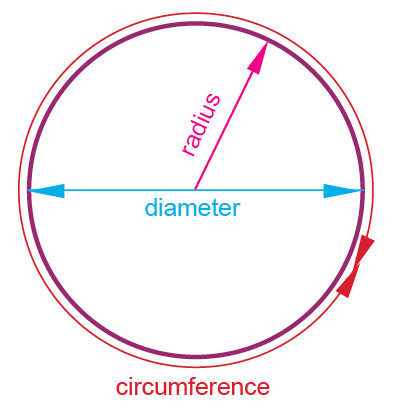
\includegraphics[scale=1]{circle.png}
\end{center}
\newpage
\section{Formulas}
The perimeter of any circle is as below:
{\Large\[C = 2\pi r\]}
Which r indicates radius. The area of any circle is as below:


{\Large\[S = \pi r^2\]}
{\Large\[\pi = 3.14159265359\]}

\section{Implementation }
Here is an implementation of Circle class in C++:



\lstset { %
  language=C++,
  backgroundcolor=\color{black!5}, % set backgroundcolor
  basicstyle=\footnotesize,% basic font setting
}


\begin{lstlisting}
class Circle {
private:
  int radius;
public:
  Circle(int r):radius(r){}
  double GetArea(){ return pi * (radius^2); }
  double Get2P(){ return 2 * pi * radius; }
  static double pi;
};

double Circle::pi=3.14159265359; 
\end{lstlisting}

\begin{center}

This marks the end of the document.
\setstretch{2} 

\color{blue}
  \textbf{{\large All Rights Reserved by Saeed All Gharaee | 2020 }} 
\end{center}
\end{document}